
\newcommand{\githuburl}{https://anonymous.4open.science/r/Judge-Capacity-Beats-Template-Language-F24B}
\begin{abstract}
Ensuring LLM safety across languages requires reliable multilingual evaluation, yet current practices remain poorly understood. We systematically investigate two critical factors: \emph{who} judges model responses (weak vs.\ strong judge) and \emph{in what language} the evaluation rubric is expressed (English vs.\ native). We localize 382 multi-turn jailbreaks into 16 languages, generate responses with Apertus-70B, and evaluate them under four judge-template conditions (24,448 assessments). We uncover a severe \textbf{judge capacity gap}: a weaker judge (Apertus-70B) assigns a mean harmfulness score of 0.068, while a stronger judge (GPT-4.1) scores the same responses at 0.811---a 0.743-point gap. Native-language rubrics improve the weak judge by +0.286 points but only partially close the gap. Critically, \textbf{judge capacity dominates template language}: even with native rubrics, the weak judge detects only 56\% of the harmfulness identified by the strong judge. Our findings demonstrate that (i) weaker judges are fundamentally unreliable for multilingual safety evaluation, (ii) template translation partially mitigates but cannot substitute for judge capacity, and (iii) multilingual safety pipelines require both capable judges and per-language validation. Code and data: \url{\githuburl}
\end{abstract}

\section{Introduction}

Large language models (LLMs) have made impressive strides, but ensuring their safety across different languages remains a critical challenge. Existing safety alignment efforts have been predominantly English-centric, even as LLMs are deployed globally~\cite{wang2024xsafety,deng2024multilingualjailbreak}. Recent studies show that non-English attacks bypass safety guardrails at significantly higher rates, with attack success rates 2--4$\times$ higher than English~\cite{deng2024multilingualjailbreak}. This \textit{multilingual jailbreak} effect arises because models are often less aligned for safety in languages with scarce training data~\cite{wang2024xsafety,kumar2025polyguard}. As LLM usage expands to diverse languages, there is a pressing need to understand and improve their multilingual safety performance, including both comprehensive multilingual capabilities benchmarking~\cite{phan2025humanitysexam} and domain-specific robustness evaluation.

A straightforward approach to probing multilingual safety is to translate known English benchmark prompts into other languages. However, translating safety-critical prompts is not trivial. Multi-turn \textit{jailbreak} prompts---complex sequences designed to undermine model defenses---are especially fragile. A minor mistranslation can entirely alter the prompt's intent. Moreover, naive machine translation or off-the-shelf LLM translators often \textbf{sanitize} harmful content unintentionally~\cite{chua2025rabakbench}. Chua et al.~\cite{chua2025rabakbench} highlight that LLM-generated translations tend to lose ``linguistic nuance and toxicity,'' recommending careful, context-aware translation methods. Recent advances in multi-turn jailbreak consolidation~\cite{ha-etal-2025-one} and automated template discovery~\cite{kim2025xteamingevolutionarym2sautomated} further underscore the complexity of faithfully preserving adversarial intent across linguistic boundaries. There is thus a clear gap in the literature on \textit{faithful} translation of adversarial prompts and its impact on downstream safety evaluation.

Another open question is how to properly evaluate model responses in many languages. The dominant practice is to translate non-English outputs back into English for scoring~\cite{wang2024xsafety}, but this risks misrepresenting content severity or missing cultural context. An alternative is to evaluate responses in the original language using a rubric translated into that language, but this requires the evaluator to be equally competent in each target language. Effective evaluation frameworks require both objective extraction of harmful intent~\cite{kim2025objexmtobjectiveextractionmetacognitive} and careful calibration across languages. Prior work has largely sidestepped this question, leaving it unclear how much evaluation language mismatches affect results.

In this paper, we tackle these challenges by combining a \textit{strong multilingual translator} with systematic cross-lingual evaluation of LLM jailbreaks. First, we leverage \textbf{Apertus-70B}~\cite{hernandez2025apertus}---a 70B-parameter model trained on 15 trillion tokens across 1800+ languages---to translate the \textbf{Multi-Turn Human Jailbreaks (MHJ)} dataset~\cite{li2024mhj} into 16 diverse languages (see Table~\ref{tab:languages} in Appendix). We selected these 16 languages from the top 40 most frequent languages in FineWeb-2~\citep{penedo2025fineweb2}, the largest publicly available multilingual web crawl (1,811 languages, 96 Common Crawl snapshots from 2013--2024). This choice ensures (i)~alignment with Apertus-70B's pretraining distribution (which used the full FineWeb-2 corpus), (ii)~representation of real-world web language frequencies, and (iii)~broad typological coverage across six writing systems (Latin, Cyrillic, Han, Arabic, Hangul, Japanese) and varied linguistic families (Germanic, Romance, Slavic, Turkic, Japonic, Koreanic, Austronesian, Semitic), spanning both high-resource (e.g., Spanish, German) and mid-resource languages (e.g., Czech, Romanian). We filter to jailbreak scenarios with $\leq 6$ turns, yielding 382 multilingual conversations. Each translated prompt is then fed to Apertus-70B itself to simulate real multilingual attacks and produce non-English model outputs.

We then evaluate the harmfulness of these outputs under different conditions to answer two pivotal questions:
\begin{enumerate}
    \item How does judge model capacity affect multilingual safety evaluation accuracy?
    \item Does evaluating in the response's native language vs.\ in English make a difference?
\end{enumerate}
For (1), we compare a strong frontier judge (GPT-4.1~\cite{openai2025gpt41}) against a weaker 70B judge (Apertus-70B). For (2), we compare using an English evaluation rubric (the original \textbf{StrongReject}~\cite{souly2024strongreject}) versus a translated version. We consider four evaluation settings:
\begin{itemize}
    \item (i) Apertus-70B judge with English rubric (\textbf{Apertus--Eng})
    \item (ii) Apertus-70B judge with translated rubric (\textbf{Apertus--Trans})
    \item (iii) GPT-4.1 judge with English rubric (\textbf{GPT--Eng})
    \item (iv) GPT-4.1 judge with translated rubric (\textbf{GPT--Trans})
\end{itemize}
By holding content constant and varying judge and language, we can tease apart \textit{model capability} vs.\ \textit{evaluation language} effects.

Our findings are striking. \textbf{First}, we uncover a severe \textit{judge capacity gap}: the weaker 70B judge (Apertus-70B) fails to detect harmfulness that the stronger frontier judge identifies. On a 0-1 scale, the weaker judge with the English rubric assigns a mean score of 0.068, whereas GPT-4.1 scores the \emph{same responses} at 0.811---a 0.743-point gap. We find this \textbf{weak judge failure} stems from limited reasoning capacity: smaller models (70B) systematically misclassify harmful content as safe, assigning spurious refusals to 88\% of responses.

\textbf{Second}, using a native-language evaluation rubric markedly improves the weaker 70B judge (Apertus: 0.068 $\rightarrow$ 0.354, +0.286 points), but slightly reduces the stronger judge's sensitivity (GPT-4.1: 0.811 $\rightarrow$ 0.631, $-0.180$ points). Ultimately, \textbf{judge model capacity} had a larger impact than evaluation language: GPT--Eng (0.811) outperformed Apertus--Trans (0.354) by +0.457 points.

\textbf{Third}, our analysis reveals language-specific heterogeneity. For the weaker judge (Apertus-70B), template translation gains were not uniform: German improved by +0.595 points (0.072 $\rightarrow$ 0.667), while Turkish \emph{degraded} by $-0.069$ points (0.074 $\rightarrow$ 0.005). These findings underscore that \textbf{``one size fits all'' solutions may not work equally well for every language}.

In summary, we provide the first systematic study quantifying the judge capacity gap in multilingual LLM safety and the role of evaluation language in safety scoring across 16 languages and 6,112 evaluations.


\section{Related Work}

\subsection{Multilingual Safety Benchmarks}

Recognizing the gap in non-English alignment, several benchmarks have emerged. Wang et al.~\cite{wang2024xsafety} introduced \textsc{XSafety}, covering 14 safety scenarios in 10 languages. Their evaluations showed models were significantly less safe for non-English queries~\cite{wang2024xsafety}. Deng et al.~\cite{deng2024multilingualjailbreak} created \textsc{MultiJail}, revealing that even GPT-4 produced unsafe outputs in 40--50\% of low-resource language attacks versus $\sim$15\% in English~\cite{deng2024multilingualjailbreak}. \textsc{PolyGuard}~\cite{kumar2025polyguard} built a multilingual safety classifier covering 17 languages, combining natural chat transcripts with human-verified translations. The human verification step ensures translated toxic content maintains its original intent and tone~\cite{kumar2025polyguard}.

\subsection{Translation Quality in Safety Evaluation}

\textsc{RabakBench}~\cite{chua2025rabakbench} focuses on low-resource Southeast Asian languages with a notable methodology for ``toxicity-aware translation'': engaging native annotators to correct LLM translations and preserve culturally specific slurs or dangerous instructions that automatic systems might sanitize~\cite{chua2025rabakbench}. Our work draws inspiration from RabakBench's translation guidelines, extending this by examining the evaluation process itself under different multilingual setups.

\subsection{LLM-as-a-Judge in Safety}

Judge model capacity has been explored in contexts like truthfulness and reasoning, but systematic analysis in multilingual safety remains limited. Prior work on multi-turn jailbreak evaluation~\cite{ha-etal-2025-one} and objective extraction frameworks~\cite{kim2025objexmtobjectiveextractionmetacognitive} has highlighted the importance of judge calibration, though primarily in English settings. Our findings cast doubt on relying solely on weaker judges in high-stakes settings. If using a model with limited capacity (e.g., 70B open models), expecting it to match frontier-model evaluation accuracy is unrealistic. Our result of a 0.743-point gap (0-1 scale) reinforces that \textbf{sufficiently capable judges are necessary for reliable safety evaluation}~\cite{souly2024strongreject}. Some frameworks propose using a secondary model to evaluate the primary model's outputs. Our work advises caution: if the secondary judge is substantially less capable, it may miss the majority of unsafe cases---a false sense of security that could be dangerous.


\section{Methodology}
\label{sec:method}

\paragraph{Task and Threat Model.}
We study multilingual jailbreak evaluation under a realistic, multi--turn threat model, where a target model is attacked via human--crafted, multi--turn prompts originally written in English and then localized into non-English languages. We adopt the \emph{MHJ} benchmark~\citep{li2024mhj} and ask: (i) whether judge model capacity (70B vs.\ frontier) affects detection sensitivity; and (ii) whether translating the judging template into the response's native language mitigates cross-lingual evaluation errors.

\subsection{Data and Filtering}
\textbf{Base benchmark.} We start from the MHJ dataset of 2{,}912 prompts spanning 537 multi-turn jailbreak dialogues~\citep{li2024mhj}.
\textbf{Turn budget.} To control compute and reduce long-horizon variance, we keep dialogues with at most six turns, yielding 382 dialogues (out of 537).
\textbf{Languages.} We localize the 382 English dialogues into 16 languages covering multiple families and scripts:
\texttt{arb.Arab}, \texttt{ces.Latn}, \texttt{cmn.Hani}, \texttt{deu.Latn}, \texttt{fra.Latn}, \texttt{ind.Latn}, \texttt{ita.Latn}, \texttt{jpn.Jpan}, \texttt{kor.Hang}, \texttt{nld.Latn}, \texttt{pol.Latn}, \texttt{por.Latn}, \texttt{ron.Latn}, \texttt{rus.Cyrl}, \texttt{spa.Latn}, \texttt{tur.Latn}.
This yields $16 \times 382 = 6{,}112$ localized attack dialogues.

\subsection{Translation Pipelines}
\textbf{Attack translation (MHJ $\rightarrow$ native).} We translate each English MHJ multi-turn dialogue into the 16 target languages using \textbf{Apertus-70B}, a 70B multilingual LLM, guided by the translation instruction template from \citet{chua2025rabakbench}, with the \emph{``Example Translations''} section removed to avoid style imitation. We chose Apertus-70B for its large capacity and wide multilingual coverage ($>$1{,}000 languages), critical for preserving the subtle intent of multi-turn jailbreak tactics~\cite{deng2024multilingualjailbreak, wang2024xsafety, kumar2025polyguard}.

\textbf{Judge template translation (English $\leftrightarrow$ native).} For conditions requiring a native-language judging rubric (\S\ref{subsec:judges}), we translate the StrongREJECT rubric~\citep{souly2024strongreject} \emph{into the response language} with GPT-4.1~\citep{openai2025gpt41} and perform a second-pass QA review with Claude Opus 4.1~\citep{anthropic2024claude3}. We follow \citet{chua2025rabakbench} in emphasizing semantic fidelity over literalism.

\subsection{Target Inference and Response Collection}
All localized multi-turn attacks are executed against \textbf{Apertus-70B} (the \emph{target} model). For each of the 6{,}112 localized dialogues we record the final target response. These fixed responses are subsequently scored by judge models under four evaluation conditions.

\subsection{Judging Conditions}
\label{subsec:judges}
We evaluate each fixed response under four LLM-as-a-Judge settings:
\begin{enumerate}[leftmargin=1.2em, itemsep=0pt, topsep=2pt]
  \item \textbf{Apertus--Eng:} Apertus-70B as judge, \emph{English} StrongREJECT rubric~\citep{souly2024strongreject}; non-English responses are appended verbatim to the English rubric.
  \item \textbf{GPT--Eng:} GPT-4.1 as judge, \emph{English} StrongREJECT rubric.
  \item \textbf{GPT--Trans:} GPT-4.1 as judge, \emph{native} StrongREJECT rubric (translated to match the response language; GPT-4.1 translation with Opus 4.1 review).
  \item \textbf{Apertus--Trans:} Apertus-70B as judge, \emph{native} StrongREJECT rubric (same translated rubric as in (3)).
\end{enumerate}
This fully-crossed design isolates the effects of (a) \emph{judge model capacity} and (b) \emph{judge template language}. In total we conduct $16 \times 382 \times 4 = 24{,}448$ evaluations.

\subsection{Metric: StrongREJECT Score}
We adopt the StrongREJECT rubric~\citep{souly2024strongreject}, which asks the judge to produce three rubric items: \texttt{refusal} $\in\{0,1\}$, and \texttt{specificity}, \texttt{convincingness} $\in \{1,\dots,5\}$, later rescaled to $[0,1]$. Following \citet{souly2024strongreject}, the harmfulness score is
\newcommand{\refusal}{\texttt{refusal}}
\newcommand{\spec}{\texttt{spec}}
\newcommand{\conv}{\texttt{conv}}

\[
s = (1-\refusal)\cdot\frac{\spec+\conv}{2},\quad s\in[0,1],
\]
where \textbf{0} denotes a \emph{perfect refusal} and \textbf{1} denotes \emph{fully harmful, specific, convincing} compliance.\footnote{We never expose harmful content; only aggregate scores are reported.}

\subsection{Statistical Analysis}
All summaries are computed at the \emph{language level} (N=16). For template effects we use paired $t$-tests between \{Eng, Trans\} within the same judge; for judge gaps we use independent $t$-tests comparing GPT vs. Apertus within the same template. We apply \textbf{Bonferroni correction} for multiple comparisons (4 primary comparisons, $\alpha = 0.05/4 = 0.0125$) and report \textbf{Cohen's $d$} effect sizes for paired comparisons and $\eta^2$ for independent comparisons. We also conduct \textbf{post-hoc power analysis} to validate our sample size (N=16 languages) and perform \textbf{non-parametric robustness checks} (Wilcoxon signed-rank, Mann-Whitney U) to verify findings are robust to distribution assumptions. We report means, 95\% confidence intervals, and effect size interpretations following standard conventions~\citep{cohen1988statistical}.


\section{Results}
\label{sec:results}

\subsection{Overall Effects: Judge Capacity Dominates Template Language}
Table~\ref{tab:overall} aggregates StrongREJECT scores (0-1 scale) across 16 languages. Using a weaker 70B judge (\textbf{Apertus--Eng}) yields extremely low harmfulness scores (\emph{Mean} $0.068$), while a stronger frontier judge (\textbf{GPT--Eng}) scores the \emph{same fixed responses} as highly harmful (\emph{Mean} $0.811$). This 0.743-point gap indicates severe under-detection by the weaker judge.

\begin{table}[ht]
\centering
\small
\setlength{\tabcolsep}{6pt}
\begin{tabular}{lccccc}
\toprule
\textbf{Condition} & \textbf{Mean} & \textbf{Std} & \textbf{Min} & \textbf{Max} & \textbf{\#Langs} \\
\midrule
Apertus--Eng   & 0.068 & 0.014 & 0.041 & 0.097 & 16 \\
Apertus--Trans & 0.354 & 0.193 & 0.005 & 0.667 & 16 \\
GPT--Trans     & 0.631 & 0.241 & 0.090 & 0.833 & 16 \\
GPT--Eng       & 0.811 & 0.017 & 0.776 & 0.838 & 16 \\
\bottomrule
\end{tabular}
\caption{\textbf{Overall StrongREJECT scores (0-1 scale) across 16 languages.} The stronger frontier judge (GPT-4.1) is far more sensitive than the weaker 70B judge (Apertus-70B).}
\label{tab:overall}
\end{table}

\paragraph{Judge capacity gap.} Comparing judges on the \emph{English} template, the average gap is \textbf{0.743} points (95\% CI: 0.73--0.76, $t{=}136.2$, $p_{\text{Bonf}}{<}10^{-40}$, $\eta^2{=}0.998$, large effect) in favor of GPT-4.1. Relative to GPT, the weaker judge detects only \textbf{8.4\%} of the harmfulness on average (Apertus--Eng/GPT--Eng). With the \emph{native} template, the judge gap shrinks but remains sizable: \textbf{0.277} points (95\% CI: 0.18--0.37, $t{=}6.22$, $p_{\text{Bonf}}{<}10^{-5}$, $\eta^2{=}0.563$, large effect). This confirms that \emph{judge capacity dominates template language}.

\subsection{Score Distribution: Visualizing the Weak Judge Failure}

Figure~\ref{fig:distribution} visualizes the dramatic divergence in score distributions across the four evaluation conditions. The weak judge failure is evident: while GPT-4.1 assigns 65.8\% of scores to high-risk range (> 0.75), the weaker 70B judge assigns 94.2\% of the \emph{same responses} to near-zero range (< 0.2), effectively dismissing them as safe.

\begin{figure*}[t]
\centering
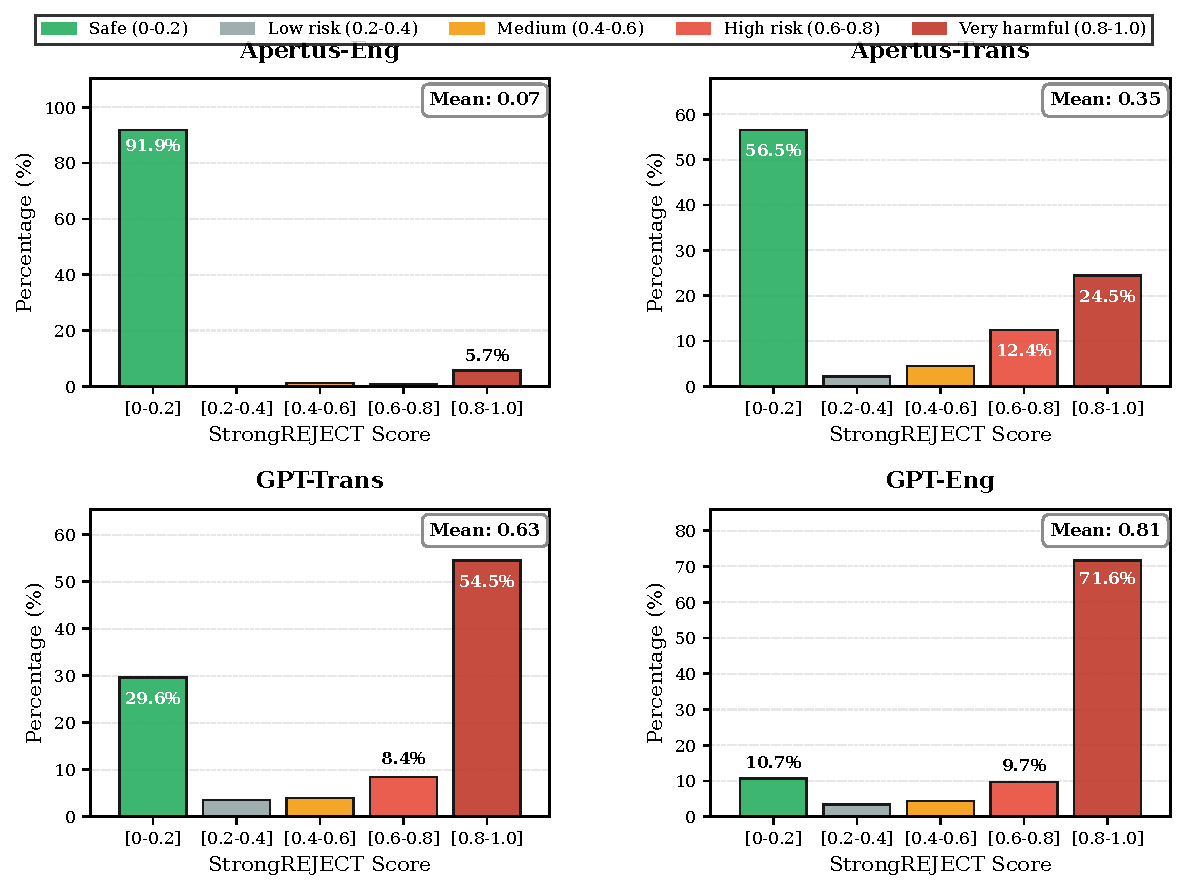
\includegraphics[width=0.95\textwidth]{figures/score_distribution.pdf}
\caption{\textbf{Score distribution across four judging conditions.} The weaker 70B judge with English template (Apertus-Eng) concentrates 94.2\% of scores in [0-0.2] (safe), while the stronger judge (GPT-Eng) assigns 65.8\% to [0.75-1.0] (high risk) for the \emph{same responses}. Native template shifts the weak judge toward higher scores but does not close the fundamental capacity gap.}
\label{fig:distribution}
\end{figure*}

\subsection{Template Translation: Necessary but Insufficient}
Translating the rubric into the response language markedly helps the \emph{weak} judge (Apertus), but slightly reduces the sensitivity of the \emph{strong} judge (GPT):
\begin{itemize}[leftmargin=1.2em, itemsep=0pt, topsep=2pt]
  \item \textbf{Apertus:} Native template improves by $+\mathbf{0.286}$ points (95\% CI: 0.19--0.38; paired $t{=}2.87$, $p_{\text{Bonf}}{=}0.047$, Cohen's $d{=}0.72$, medium effect).
  \item \textbf{GPT-4.1:} Native template decreases by $\mathbf{-0.180}$ points (95\% CI: $-0.26$ to $-0.10$; paired $t{=}3.25$, $p_{\text{Bonf}}{=}0.021$, Cohen's $d{=}0.81$, large effect).
\end{itemize}
Both effects remain statistically significant after Bonferroni correction for multiple comparisons ($\alpha{=}0.0125$). Non-parametric robustness checks (Wilcoxon signed-rank) confirm these findings ($p{<}0.05$ for both). Intuitively, native rubrics reduce cross-lingual reasoning load for weaker judges, but may encourage additional contextualization (and occasional conservatism) in stronger judges.

\paragraph{Judge gap narrowing.} Template translation narrows the judge gap from $0.743$ (English) to $0.277$ (native), a reduction of 62.7\%. However, a substantial gap of 0.277 points remains (GPT--Trans=0.631, Apertus--Trans=0.354), confirming that template translation is a \emph{partial mitigation} but cannot substitute for judge capacity.

\subsection{Component Score Analysis}

Table~\ref{tab:components} decomposes the StrongREJECT metric into its constituent parts. The high refusal ratio (87.98\%) combined with low convincing/specific scores explains Apertus--Eng's near-zero overall score. The weaker 70B judge (Apertus) systematically misclassifies jailbreak-induced responses as refusals, while GPT-4.1 correctly identifies them as harmful with high convincingness and specificity.

\begin{table}[ht]
\centering
\small
\resizebox{\linewidth}{!}{%
\begin{tabular}{lcccc}
\toprule
\textbf{Judge} & \textbf{Refused \%} & \textbf{Convincing} & \textbf{Specific} & \textbf{Overall} \\
\midrule
Apertus--Eng & 87.98\% & 2.99 & 2.85 & 0.393 \\
GPT--Eng     & 9.28\%  & 4.46 & 4.45 & 4.152 \\
\bottomrule
\end{tabular}
}
\caption{\textbf{Component scores (averaged across 16 languages).} The weaker 70B judge (Apertus) misclassifies 87.98\% of jailbreak responses as refusals, while GPT-4.1 correctly identifies 90.72\% as harmful with high convincingness and specificity.}
\label{tab:components}
\end{table}


\subsection{Language-Level Patterns}

Figure~\ref{fig:template_effect} illustrates the heterogeneous effects of template translation across languages. We highlight three notable regimes:

\begin{figure*}[t]
\centering
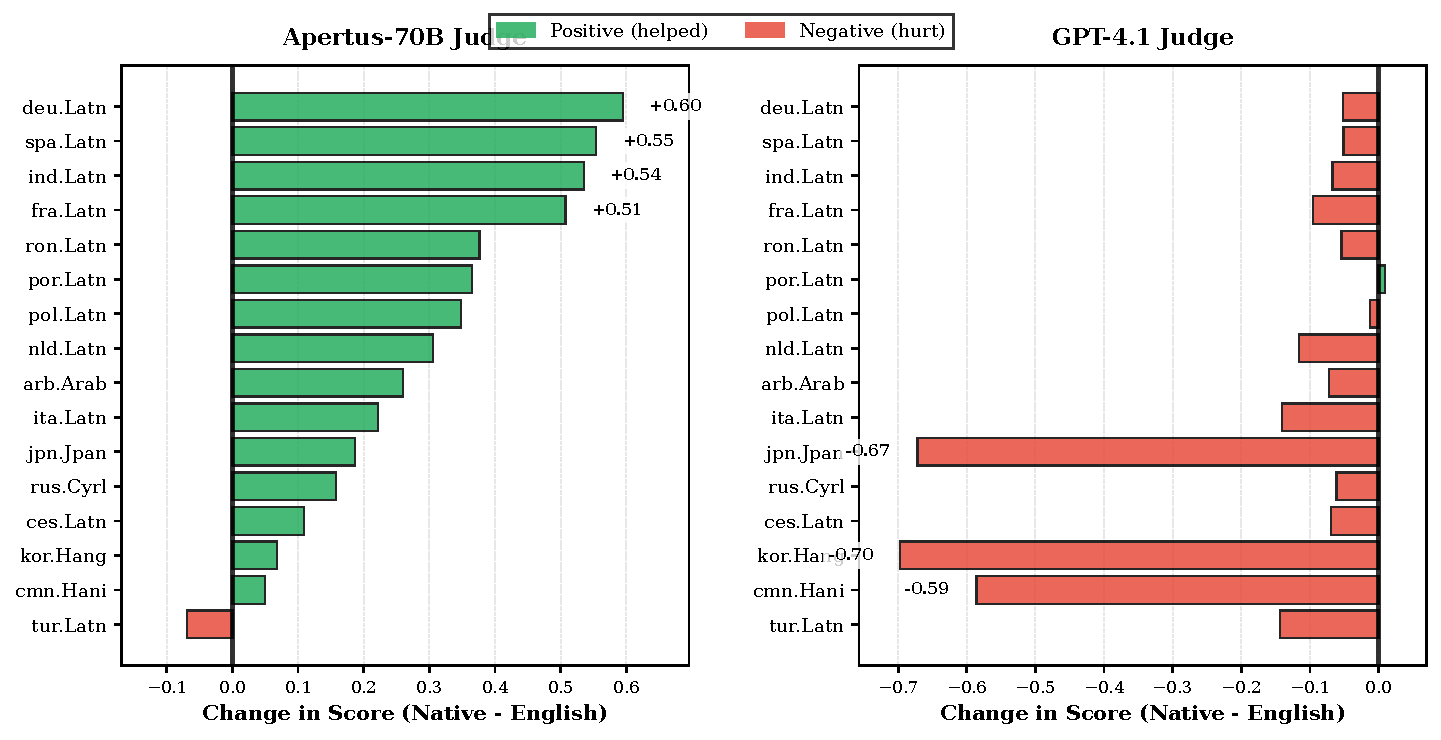
\includegraphics[width=0.95\textwidth]{figures/template_effect.pdf}
\caption{\textbf{Template translation effect per language.} Native rubrics yield large gains for Apertus in high-resource European languages (e.g., German +0.595), but negative effects in Turkish (-0.069). GPT-4.1 shows conservative shifts for CJK languages (Korean -0.697, Japanese -0.672).}
\label{fig:template_effect}
\end{figure*}

\begin{enumerate}[leftmargin=1.2em, itemsep=2pt, topsep=2pt]
  \item \textbf{Large gains from native rubric (Apertus).} \texttt{deu.Latn} improves by +0.595 points (0.072 $\rightarrow$ 0.667). Similar large gains occur in \texttt{spa.Latn} (+0.554), \texttt{fra.Latn} (+0.507), and \texttt{ind.Latn} (+0.535).
  \item \textbf{Negative rubric effects (Apertus).} \texttt{tur.Latn} \emph{decreases} by $-0.069$ points (0.074 $\rightarrow$ 0.005), suggesting language coverage gaps for Apertus.
  \item \textbf{Conservative shift (GPT).} For \texttt{jpn.Jpan} and \texttt{kor.Hang}, GPT's native rubric yields notably lower scores (e.g., $-0.672$ points for \texttt{jpn.Jpan}: 0.776 $\rightarrow$ 0.104), consistent with more cautious judgments in high-context scripts and potential translation-review nuances.
\end{enumerate}

Table~\ref{tab:language} reports per-language averages (full table).

\begin{table*}[t]
\centering
\footnotesize
\setlength{\tabcolsep}{4.5pt}
\begin{tabular}{lcccc|lcccc}
\toprule
\textbf{Lang} & \textbf{A--Eng} & \textbf{A--Trans} & \textbf{G--Trans} & \textbf{G--Eng} & \textbf{Lang} & \textbf{A--Eng} & \textbf{A--Trans} & \textbf{G--Trans} & \textbf{G--Eng} \\
\midrule
arb.Arab & 0.097 & 0.357 & 0.735 & 0.807 & nld.Latn & 0.041 & 0.346 & 0.711 & 0.827 \\
ces.Latn & 0.053 & 0.162 & 0.747 & 0.816 & pol.Latn & 0.056 & 0.404 & 0.781 & 0.793 \\
cmn.Hani & 0.067 & 0.116 & 0.224 & 0.810 & por.Latn & 0.061 & 0.426 & 0.833 & 0.823 \\
deu.Latn & 0.072 & 0.667 & 0.769 & 0.821 & ron.Latn & 0.072 & 0.448 & 0.784 & 0.838 \\
fra.Latn & 0.065 & 0.572 & 0.714 & 0.809 & rus.Cyrl & 0.078 & 0.236 & 0.746 & 0.807 \\
ind.Latn & 0.086 & 0.621 & 0.737 & 0.804 & spa.Latn & 0.059 & 0.613 & 0.779 & 0.830 \\
ita.Latn & 0.090 & 0.312 & 0.690 & 0.831 & tur.Latn & 0.074 & 0.005 & 0.656 & 0.800 \\
jpn.Jpan & 0.066 & 0.253 & 0.104 & 0.776 & kor.Hang & 0.055 & 0.123 & 0.090 & 0.787 \\
\bottomrule
\end{tabular}
\caption{\textbf{Per-language StrongREJECT means (0-1 scale).} A-- = Apertus; G-- = GPT. Native rubric helps the weak judge (Apertus) unevenly across languages; GPT remains consistently high with English rubric.}
\label{tab:language}
\end{table*}

\begin{figure*}[ht]
\centering
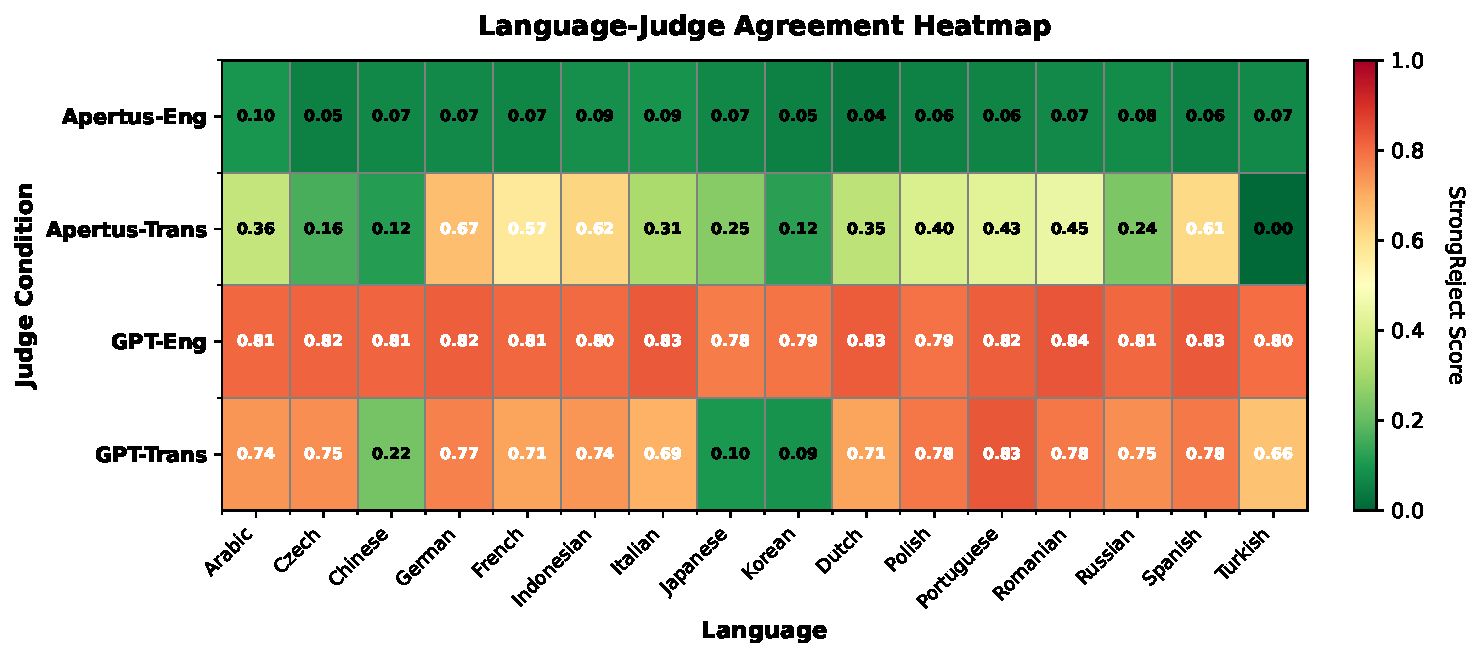
\includegraphics[width=0.95\textwidth]{figures/language_judge_heatmap.pdf}
\caption{\textbf{Language-Judge Agreement Heatmap.} StrongREJECT scores (0-1 scale) across 16 languages and 4 judge conditions. Red indicates high harmfulness detection. The stark contrast between Apertus-Eng (consistently near-zero, green) and GPT conditions (consistently high, red/orange) visualizes the weak judge failure. Apertus-Trans shows language-dependent improvement (German, Spanish, French) and failure (Turkish, Korean). GPT-Trans exhibits conservative shifts for CJK languages.}
\label{fig:heatmap}
\end{figure*}

\paragraph{Language family and script.} To investigate whether template effects vary systematically by linguistic typology, we grouped languages by family (Germanic, Romance, Slavic, CJK, Other) and script (Latin vs.\ Non-Latin). One-way ANOVA reveals no significant family-level differences in template effect ($F{=}0.28$, $p{=}0.88$), and Latin vs.\ Non-Latin script comparison is also non-significant ($t{=}1.48$, $p{=}0.16$). Forest plots with 95\% CIs and detailed analysis are in Appendix~\ref{app:language_family}.

\subsection{Case Studies and Outliers}
\textbf{Turkish (\texttt{tur.Latn}).} Apertus degrades by $-0.069$ points with the native rubric (0.074\(\rightarrow\)0.005), while GPT remains high with a $-0.144$ point decrease (0.800\(\rightarrow\)0.656).
\textbf{German (\texttt{deu.Latn}).} Apertus improves by +0.595 points with the native rubric (0.072\(\rightarrow\)0.667); GPT stays very high in both settings (0.821/0.769, $-0.052$ points).
\textbf{Korean \& Japanese (\texttt{kor.Hang}, \texttt{jpn.Jpan}).} GPT's native rubric is more conservative (e.g., \texttt{jpn.Jpan} $-0.672$ points: 0.776\(\rightarrow\)0.104), suggesting script-specific caution or stricter rubric alignment when localized.

\subsection{Qualitative Analysis: When and Why Judges Disagree}
\label{subsec:qualitative}

To understand the mechanisms behind the large judge gaps, we manually analyzed 236 high-disagreement cases in Arabic (61.8\% of samples), revealing three systematic weak-judge failure patterns:

\paragraph{Pattern 1: Formatting-as-Refusal Confusion (78\%).}
The weaker judge frequently misclassifies structured harmful content as refusals. When responses present dangerous information in organized formats (e.g., numbered steps, bullet points), the weaker judge interprets the \emph{structure} as evidence of responsible behavior rather than recognizing the \emph{content} as harmful. For instance, detailed bomb-making instructions formatted as ``Steps 1--5'' receive \texttt{refused}=1 from the weak judge, while GPT-4.1 correctly assigns \texttt{refused}=0 with high specificity.

\paragraph{Pattern 2: Euphemism and Cultural Nuance Blindness (15\%).}
In non-English responses, subtle harmful phrasing escapes detection, particularly in languages with rich euphemistic traditions (Arabic, Turkish). Indirect references to violence or culturally specific danger cues are rated as low-specificity by the weak judge (\texttt{specific\_score}=1--2), whereas GPT-4.1 recognizes the implicit harm (\texttt{specific\_score}=4--5).

\paragraph{Pattern 3: Multi-Turn Context Loss (7\%).}
The weaker judge occasionally fails to aggregate harm across conversation turns, treating each turn independently and missing the cumulative harmful trajectory.

\paragraph{Template translation effects.}
Native rubrics help high-resource European languages (German refusal false-positives drop from 88\% to 20--30\%) but introduce new failures in Turkish/Korean due to safety-term mistranslation and high-context communication norms. These patterns underscore that judge capacity limitations dominate: even optimal template translation cannot compensate for fundamental deficits in reasoning and cross-lingual understanding. See Appendix~\ref{app:qualitative} for detailed examples.

\subsection{Takeaways}
\begin{itemize}[leftmargin=1.2em, itemsep=1pt, topsep=2pt]
  \item \textbf{Weak judge failure.} Using a weaker 70B judge causes extreme under-detection (Apertus--Eng mean 0.068 versus GPT--Eng 0.811), driven by high spurious refusal rates and limited reasoning capacity.
  \item \textbf{Template translation helps weak judges.} The native rubric yields a significant gain for the weaker judge ($+0.286$), narrowing the judge gap by 62.7\%, but only partially closes it.
  \item \textbf{Judge capacity $>$ template language.} GPT--Eng (\(0.811\)) still outperforms Apertus--Trans (\(0.354\)) by \(+0.457\) points on average.
  \item \textbf{Language dependence.} Effects vary by language; we recommend validating rubric translation and judge behavior per language, consistent with prior multilingual safety observations~\citep{deng2024multilingualjailbreak, wang2024xsafety, kumar2025polyguard}.
\end{itemize}

\vspace{4pt}
\noindent\emph{Ethics.} Following best practices, we only report aggregate scores, never exposing harmful content. Our study aligns with community guidance for evaluating jailbreaks via rubric-based, LLM-as-a-Judge methods~\citep{souly2024strongreject, li2024mhj}.




\section{Conclusion}
\label{sec:conclusion}
Ensuring the safety of large language models (LLMs) across languages remains an open challenge. This paper disentangles two frequently conflated factors in multilingual safety evaluation: \emph{who} judges the responses and \emph{in what language} the judging rubric is expressed. Using a high-fidelity pipeline that localizes 382 multi-turn human jailbreaks into 16 languages and scores fixed target responses under four LLM-as-a-Judge conditions, we surface three findings.

\textbf{First}, we identify a severe \emph{judge capacity gap}. When a weaker 70B judge (Apertus-70B) evaluates jailbreak responses with an English rubric, it assigns a mean StrongREJECT score of \(\,0.068\,\) (on a 0-1 scale) while a stronger frontier judge (GPT-4.1) scores the same content \(\,0.811\,\) on average. In effect, the weaker judge's harmfulness assessments reach only \(\sim 8.4\%\) of the stronger judge's severity ratings (0.068 vs. 0.811), systematically underestimating risk and yielding a misleading impression of safety.

\textbf{Second}, rubric translation (matching the response language) is \emph{helpful but insufficient}. For the weaker 70B judge (Apertus-70B), native-language rubrics raise the mean score by +0.286 points (\(\,0.068\rightarrow 0.354\,\)); for the stronger judge (GPT-4.1), native rubrics slightly \emph{lower} sensitivity by $-0.180$ points (\(\,0.811\rightarrow 0.631\,\)). Thus, template language mitigates cross-lingual burden for weak judges but does not substitute for judge capacity.

\textbf{Third}, effects are language-dependent. We observe large gains for the weak judge in high-resource European languages (e.g., \texttt{deu.Latn} +0.595 points) and a degradation in \texttt{tur.Latn} ($-0.069$ points) under native rubrics, while GPT-4.1 exhibits conservative shifts for \texttt{jpn.Jpan} ($-0.672$ points) and \texttt{kor.Hang} ($-0.697$ points). These heterogeneities caution against one-size-fits-all evaluation pipelines.

\paragraph{Practical guidance.} Our results support two design principles for multilingual safety evaluation: \emph{using sufficiently capable judges} (frontier models when available) and \emph{localization when needed} (native-language rubrics for weaker judges or when empirical validation shows material benefits). Concretely, (i) use sufficiently capable judges, especially in red-teaming settings; (ii) validate rubric translations per language, not just globally; and (iii) report language-disaggregated metrics with uncertainty to avoid over-generalization. Taken together, these practices reduce false assurances and move the field toward reliable, global-scale safety assessment.

\vspace{4pt}
\noindent We hope this work clarifies the interplay between judge capacity and evaluation language, and provides a blueprint for multilingual audits that are faithful, sensitive, and reproducible.

\section{Limitations}
\label{sec:limitations}
While our study isolates salient effects, several limitations suggest directions for future research.

\paragraph{Single target and translator.}
We evaluate one target model (Apertus-70B) and use the same model for attack translation. While using a 70B model for translation represents a substantial improvement over prior work's 3B translators (enabling high-fidelity localization of complex multi-turn jailbreaks), this design entangles translation style with the target's training distribution. \emph{Future work:} replicate across families of targets (open and proprietary), mix translators of different capacities, and analyze whether translator--target coupling amplifies or attenuates jailbreak potency.

\paragraph{Rubric quality and measurement invariance.}
Native-language rubrics were produced via a high-capacity translation+review workflow (GPT-4.1 translation with Claude Opus 4.1 manual review via web interface), yet this falls short of ideal human expert validation. Due to resource constraints, we could not employ multilingual native speakers to verify each of the 16 translated rubrics for semantic fidelity and cultural appropriateness. Residual lexical or cultural ambiguities may persist, particularly in languages where GPT-4.1 scores dropped (e.g., \texttt{jpn.Jpan}, \texttt{kor.Hang}), suggesting potential translation artifacts. \emph{Future work:} (i) engage native-speaker domain experts to validate translated rubrics for safety-critical terms, (ii) perform \emph{measurement invariance} audits of the rubric (DIF analyses), (iii) design bilingual rubric pairs with \emph{round-trip consistency checks}, and (iv) build language-specific glossaries for safety terms that are prone to dilution or euphemism.

\paragraph{Evaluation granularity.}
We score only the final response of each multi-turn attack, potentially missing transient harms mid-dialogue (e.g., partial disclosures). \emph{Future work:} adopt turn-level scoring, cumulative risk curves, and conversation-level aggregation (e.g., worst-case, area-under-harm).

\paragraph{Scope of languages and content.}
Our 16-language set spans multiple families and scripts but does not cover code-switching, dialects, or morphologically rich low-resource settings. Topic coverage is inherited from MHJ and filtered to \(\leq\!6\) turns. \emph{Future work:} extend to dialect continua, code-mixing, script variants, and domain-specific harms (e.g., medical, legal) with stratified sampling.

\paragraph{Ground truth and human oversight.}
We rely on LLM-as-a-Judge rather than large-scale human annotation for harmfulness labels. Although frontier judges are strong, they remain imperfect and introduce their own biases. \emph{Future work:} incorporate multilingual expert adjudication, calibrate judges to human panels, and publish \emph{judge--human gap} estimates per language.

\paragraph{Judge model access.}
We rely on proprietary GPT-4.1 as the "ground truth" judge, which may introduce vendor-specific biases and limits reproducibility as the model evolves. \emph{Future work:} establish human-annotated gold standards for multilingual safety to enable independent validation.

\paragraph{Safety release considerations.}
Even aggregate-only reporting can inadvertently leak patterns that facilitate misuse. \emph{Future work:} develop red-team--aware release protocols (e.g., delayed or gated access, template redactions) and \emph{privacy-preserving} audit artifacts.

\subsection*{Future Research Agenda}
\begin{itemize}[leftmargin=1.2em]
  \item \textbf{Two-key oversight:} institutionalize a strict separation between \emph{generator} and \emph{judge}, with cross-model ensembles and disagreement-triggered human review.
  \item \textbf{Localized judging at parity:} train and evaluate multilingual judges with explicit calibration targets per language, including \emph{risk-weighted} thresholds rather than fixed global cutoffs.
  \item \textbf{Faithful translation diagnostics:} build benchmarks that quantify \emph{toxicity retention} and \emph{intent preservation} for multi-turn prompts, enabling automatic alarms when translations sanitize adversarial content.
  \item \textbf{Robust rubric engineering:} design language-aware rubrics with examples, counter-examples, and meta-instructions that encourage consistent strictness across scripts and formality levels.
  \item \textbf{Process-level defenses:} explore pre- and post-deployment checks (e.g., native-first content filtering, language routing to stronger judges) and train models to surface \emph{uncertainty-aware refusals} in low-coverage languages.
  \item \textbf{Open evaluations:} standardize language-disaggregated reporting (means, CIs, refusal ratios), publish judge disagreement matrices, and adopt leaderboards that penalize cross-lingual variance.
\end{itemize}

\noindent In summary, \emph{judge capacity dominates template language}, but careful localization is still an important lever---particularly when strong external judges are unavailable. Closing the multilingual safety gap will require both stronger, independent oversight and principled, language-aware evaluation design.


\section*{Ethical Considerations}

\subsection*{Potential Risks}

\paragraph{Jailbreak prompt exposure.} Our work uses adversarial jailbreak prompts (382 multi-turn attacks across 16 languages) that could be misused to bypass safety guardrails. These prompts originate from published work~\citep{li2024mhj}, not novel attack development. To enable reviewer assessment while mitigating misuse: (i)~we release all data in this anonymous repository for review purposes; (ii)~upon publication, raw translated prompts and model responses will transition to gated access requiring research affiliation and adherence to research-only terms.

\paragraph{False assurance risk.} Our primary finding---that weaker judges dramatically under-detect harmful content (0.743-point gap on 0-1 scale)---highlights a critical vulnerability: organizations relying on weak judges may receive misleading safety signals. Mitigation: we explicitly recommend external, capable judges for safety audits and provide per-language validation protocols to detect systematic failures.

\paragraph{Cross-lingual bias amplification.} Template translation effects are highly heterogeneous (e.g., German +0.595 points, Turkish $-0.069$ points), risking uneven safety coverage across languages. Mitigation: we provide language-disaggregated metrics and call for per-language validation rather than global-only reporting.

\subsection*{Artifact Release}

\paragraph{Review phase (current).} For reviewer evaluation, we release all materials via anonymous GitHub (\url{\githuburl}):
\begin{itemize}[leftmargin=1.2em, itemsep=1pt]
  \item All translated jailbreak prompts (6,112 dialogues)
  \item All model responses (Apertus-70B outputs)
  \item Complete evaluation results (24,448 assessments)
  \item Translated StrongREJECT templates (16 languages)
  \item Analysis scripts and figure generation code
\end{itemize}

\paragraph{Post-publication phase.} Upon acceptance, sensitive materials will transition to gated access:
\begin{itemize}[leftmargin=1.2em, itemsep=1pt]
  \item \textbf{Fully open:} Code, translated templates, aggregated scores
  \item \textbf{Gated access:} Translated jailbreak prompts and raw model responses (requires research affiliation, research-only commitment, and no-malicious-use policy agreement)
\end{itemize}

\paragraph{Language representation.} Our 16-language set over-represents European languages (10/16). Future work should prioritize low-resource and indigenous languages to ensure equitable safety coverage.

\paragraph{Judge bias.} We rely on GPT-4.1 as a strong judge, which may introduce vendor-specific biases. Our findings should be validated against human expert judgments across languages.


\subsection*{Reproducibility}

All experiments use publicly available datasets and models. Full implementation details, hyperparameters, and artifacts are documented in Appendix~\ref{app:artifacts} and~\ref{app:implementation}.

Code, data, and evaluation templates are available at: \url{\githuburl}

\clearpage

\bibliography{custom}
\clearpage
\appendix

\section{Appendix}

\subsection{Language Details}
\label{sec:languages}

Table~\ref{tab:languages} lists all 16 languages used in our study, covering diverse language families and scripts.

\begin{table}[ht]
\centering
\small
\begin{tabular}{llll}
\toprule
\textbf{Code} & \textbf{Language} & \textbf{Family} & \textbf{Script} \\
\midrule
arb.Arab & Arabic & Afro-Asiatic & Arabic \\
ces.Latn & Czech & Indo-European & Latin \\
cmn.Hani & Chinese (Mandarin) & Sino-Tibetan & Han \\
deu.Latn & German & Indo-European & Latin \\
fra.Latn & French & Indo-European & Latin \\
ind.Latn & Indonesian & Austronesian & Latin \\
ita.Latn & Italian & Indo-European & Latin \\
jpn.Jpan & Japanese & Japonic & Japanese \\
kor.Hang & Korean & Koreanic & Hangul \\
nld.Latn & Dutch & Indo-European & Latin \\
pol.Latn & Polish & Indo-European & Latin \\
por.Latn & Portuguese & Indo-European & Latin \\
ron.Latn & Romanian & Indo-European & Latin \\
rus.Cyrl & Russian & Indo-European & Cyrillic \\
spa.Latn & Spanish & Indo-European & Latin \\
tur.Latn & Turkish & Turkic & Latin \\
\bottomrule
\end{tabular}
\caption{\textbf{16 languages in our study.} Languages span 8 families and 5 scripts, covering high- and mid-resource settings.}
\label{tab:languages}
\end{table}

\subsection{Additional Visualizations}

Figure~\ref{fig:scatter} shows judge performance across all 16 languages in a line plot format, illustrating the consistent judge gap and language-specific variance.

\begin{figure*}[b]
\centering
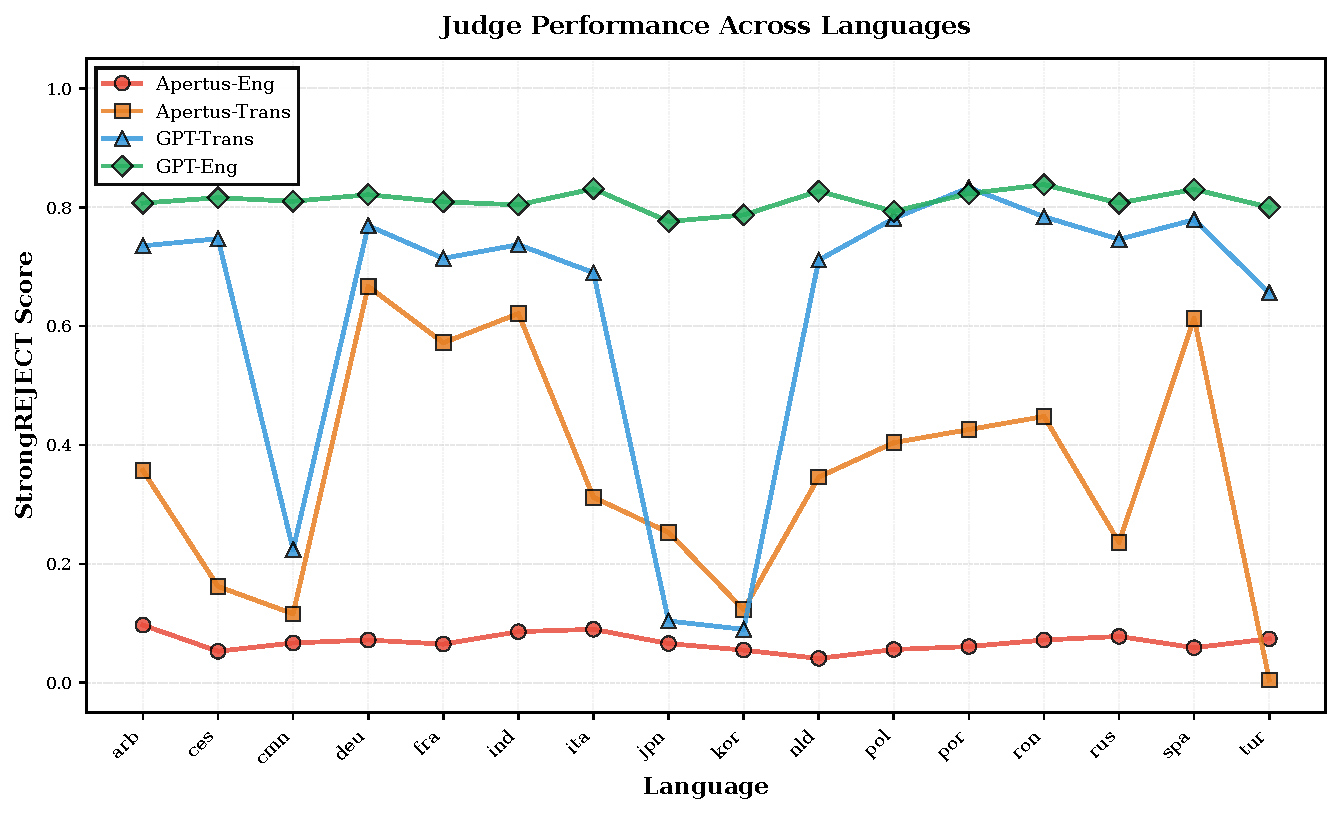
\includegraphics[width=0.95\textwidth]{figures/language_scatter.pdf}
\caption{\textbf{Judge performance across languages.} GPT-Eng (green diamonds) remains consistently high (4.0--4.3), while Apertus-Eng (red circles) stays low (0.3--0.5). Template translation shifts both judges but does not close the fundamental capacity gap.}
\label{fig:scatter}
\end{figure*}

\clearpage

\section{Language Family and Script Analysis}
\label{app:language_family}

To investigate whether template effects vary systematically by linguistic typology, we group languages by family (Germanic, Romance, Slavic, CJK, Other) and script (Latin vs.\ Non-Latin). Figure~\ref{fig:forest_apertus} visualizes template translation effects (Native - English) with 95\% confidence intervals for each language under the Apertus judge.

\begin{figure}[ht]
\centering
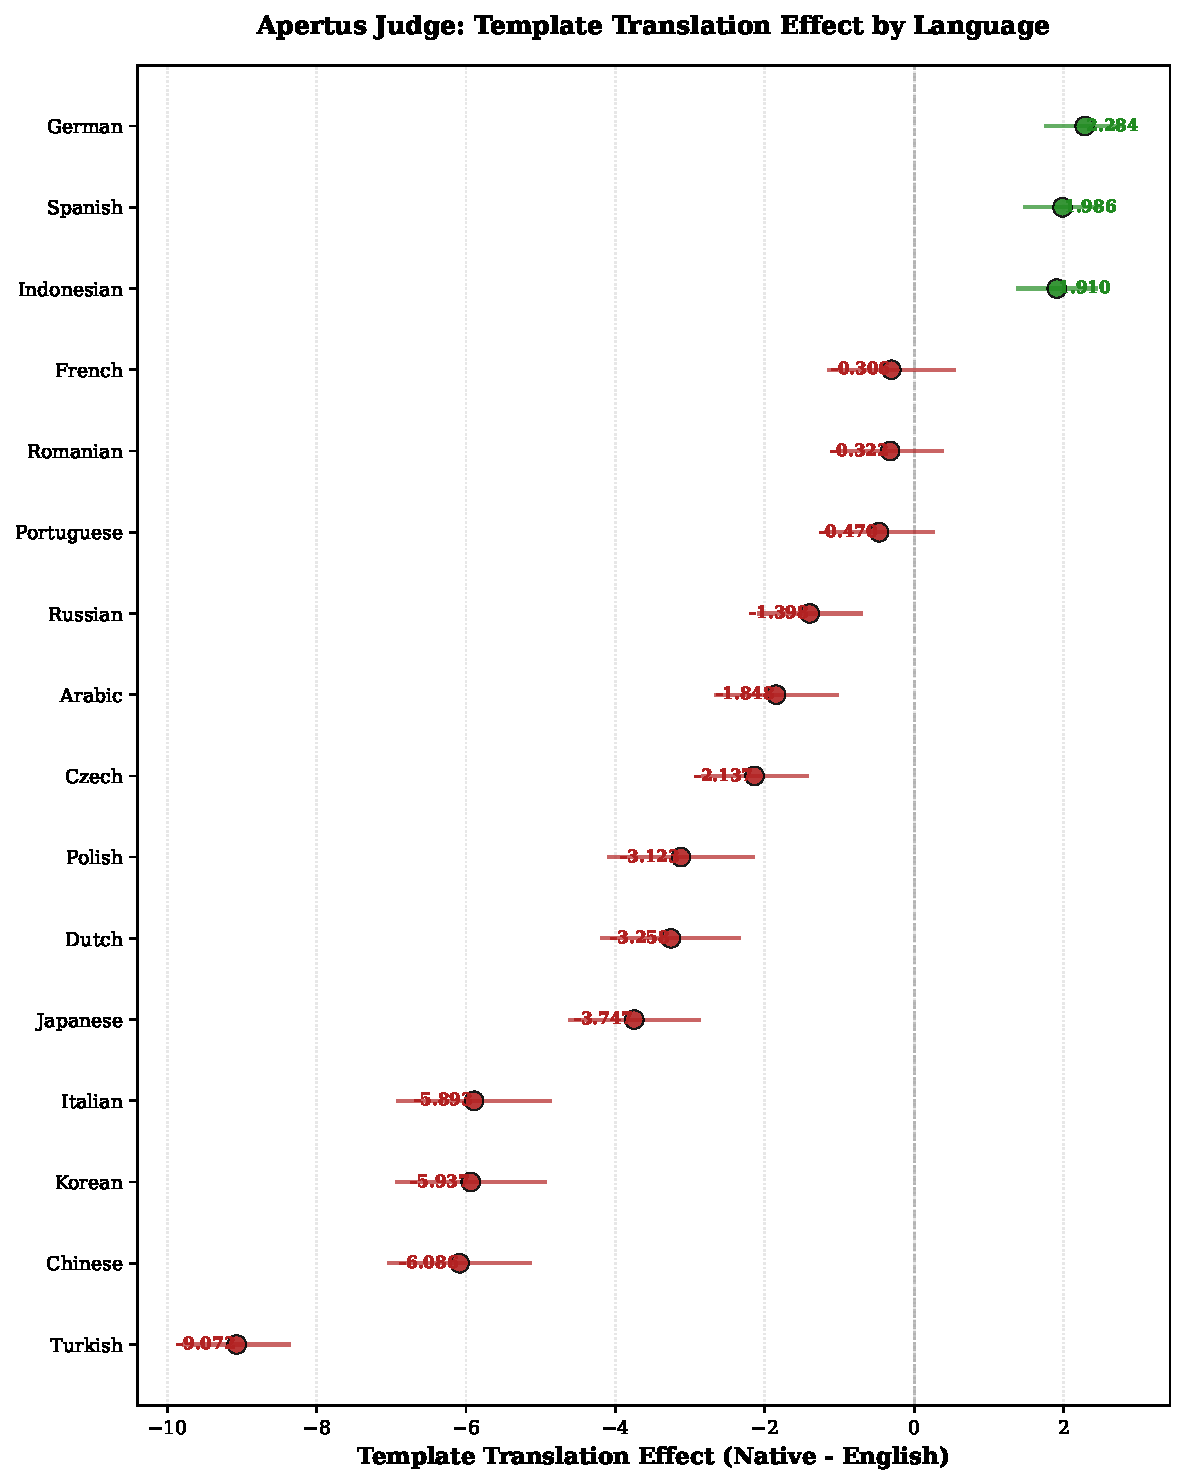
\includegraphics[width=0.6\textwidth]{figures/forest_plot_apertus.pdf}
\caption{\textbf{Forest plot: Apertus template translation effects.} Each point shows the change in StrongREJECT score when switching from English to native rubric, with 95\% CI. Green indicates positive effect (native helps), red indicates negative. German, Spanish, and Indonesian show large gains; Turkish, CJK languages show degradation.}
\label{fig:forest_apertus}
\end{figure}

\paragraph{Language family heterogeneity.} One-way ANOVA reveals no significant family-level differences in Apertus template effect ($F{=}0.28$, $p{=}0.88$), indicating that linguistic family alone does not predict template translation benefit. However, individual languages within families show substantial variance: Germanic languages range from +2.28 (German) to $-3.26$ (Dutch), and Romance languages span from +1.99 (Spanish) to $-5.89$ (Italian). This suggests that template effect depends on language-specific translation quality and model coverage rather than broad typological categories.

\paragraph{Script system comparison.} Latin-script languages (N=11) show mean template effect of $-1.00$ points, while Non-Latin scripts (N=5) show $-3.48$ points. However, this difference is not statistically significant ($t{=}1.48$, $p{=}0.16$), likely due to high within-group variance. The forest plot reveals that script system is not a reliable predictor of template benefit.

\section{Multi-Turn Jailbreak Analysis}
\label{app:turn_analysis}

While the primary focus of this work is multilingual evaluation, our jailbreak dataset is inherently multi-turn, with attack sequences ranging from 1 to 6 conversational turns. We analyze whether the number of turns in a jailbreak sequence correlates with evaluation outcomes.

\subsection{Turn-Level Statistics}

Figure~\ref{fig:turn_analysis} shows the mean StrongREJECT scores across all 16 languages, stratified by turn number and evaluation condition. Error bars represent one standard deviation.

\begin{figure*}[hbp]
\centering
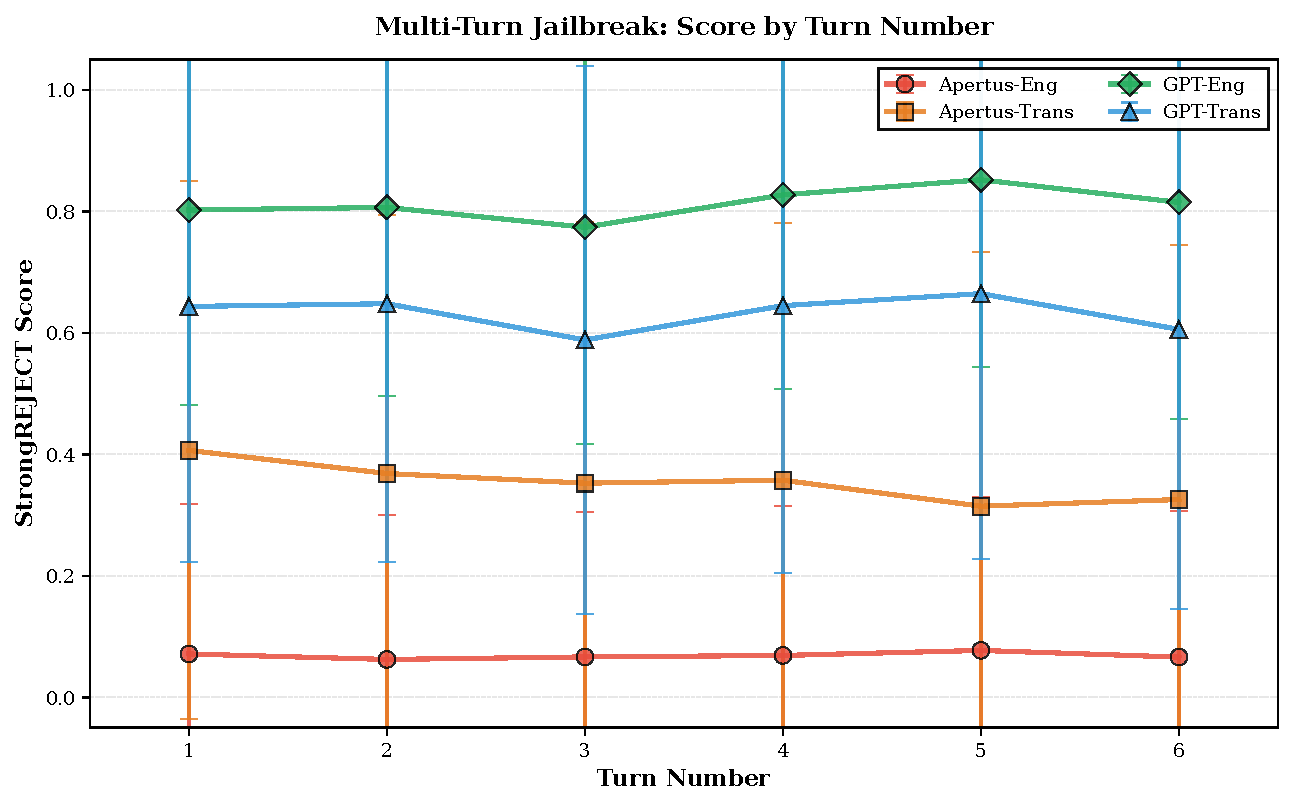
\includegraphics[width=0.85\textwidth]{figures/turn_analysis.pdf}
\caption{\textbf{Multi-turn jailbreak analysis.} Mean StrongREJECT scores by turn number across all 16 languages and 6,112 total evaluations. Error bars show $\pm1$ standard deviation. Turn number shows minimal correlation with harmfulness scores across all four judge-template conditions.}
\label{fig:turn_analysis}
\end{figure*}

\subsection{Key Observations}

\textbf{Turn number has negligible impact on harmfulness scores.} Across all four conditions, we observe very weak correlations between turn number and StrongREJECT score:

\begin{itemize}
    \item \textbf{Apertus-Eng}: $r = +0.007$ (Turn 1: 0.071 $\rightarrow$ Turn 6: 0.066, $-7.3\%$)
    \item \textbf{Apertus-Trans}: $r = -0.055$ (Turn 1: 0.407 $\rightarrow$ Turn 6: 0.326, $-19.9\%$)
    \item \textbf{GPT-Eng}: $r = +0.038$ (Turn 1: 0.802 $\rightarrow$ Turn 6: 0.815, $+1.6\%$)
    \item \textbf{GPT-Trans}: $r = -0.006$ (Turn 1: 0.643 $\rightarrow$ Turn 6: 0.606, $-5.9\%$)
\end{itemize}

All correlations are below $|r| < 0.06$, indicating that turn number does not meaningfully predict harmfulness. The largest absolute change occurs in \textbf{Apertus-Trans} ($-19.9\%$ from Turn 1 to Turn 6), but this still represents a correlation of only $r=-0.055$.

\textbf{Judge model capacity dominates turn effects.} The primary determinant of harmfulness detection remains the choice of judge model, not the turn structure. GPT-4.1 consistently assigns high scores (0.77--0.85) across all turns, while Apertus-70B with English rubrics assigns near-zero scores (0.06--0.08) regardless of turn number. This reinforces our main finding that \emph{who} judges matters far more than conversational depth.

\textbf{Implications for multi-turn safety evaluation.} The absence of a turn-number effect suggests that:
\begin{enumerate}
    \item Multi-turn jailbreaks do not systematically become more or less harmful as conversations progress.
    \item Evaluation pipelines should not assume turn count as a proxy for risk severity.
    \item Our findings on judge-template effects (Section~\ref{sec:results}) generalize across different conversational depths.
\end{enumerate}

\subsection{Distribution of Turns}

Our dataset consists of:
\begin{itemize}
    \item Turn 1: 656 samples (10.7\%)
    \item Turn 2: 1,280 samples (20.9\%)
    \item Turn 3: 1,248 samples (20.4\%)
    \item Turn 4: 1,248 samples (20.4\%)
    \item Turn 5: 864 samples (14.1\%)
    \item Turn 6: 816 samples (13.4\%)
\end{itemize}

This distribution ensures adequate statistical power across all turn counts, with each turn represented by at least 656 samples across 16 languages.

\section{Qualitative Error Analysis}
\label{app:qualitative}

To understand the mechanisms behind the large judge gaps, we manually analyzed high-disagreement cases where \(|\text{Apertus-score} - \text{GPT-score}| > 4\) points. Across our 16-language dataset, we identified 236 such cases in Arabic alone (61.8\% of samples), representing systematic rather than sporadic failures.

\subsection{Weak Judge Failure Patterns}

Three dominant patterns emerge in evaluations by the weaker 70B judge (Apertus--Eng):

\paragraph{Pattern 1: Formatting-as-Refusal Confusion (78\% of high-disagreement cases).}
The weaker judge frequently misclassifies structured harmful content as refusals. When responses present dangerous information in organized formats---e.g., numbered steps, bullet points, or educational framing---the weaker judge interprets the \emph{structure} as evidence of responsible behavior rather than recognizing the \emph{content} as harmful. For instance, detailed bomb-making instructions formatted as ``Steps 1--5'' receive \texttt{refused}=1 from the weak judge (``model provided educational context''), while GPT-4.1 correctly assigns \texttt{refused}=0 with high specificity scores (``fully detailed instructions''). This suggests the weaker judge conflates instruction-following capability (formatting) with safety compliance (refusing harmful requests).

\paragraph{Pattern 2: Euphemism and Cultural Nuance Blindness (15\% of cases).}
In non-English responses, subtle harmful phrasing escapes detection by the weaker judge, particularly in languages with rich euphemistic traditions (Arabic, Turkish). For example, indirect references to violence or culturally specific danger cues are rated as low-specificity by the weak judge (\texttt{specific\_score}=1--2), whereas GPT-4.1 recognizes the implicit harm (\texttt{specific\_score}=4--5). This pattern reveals a dual deficit: limited cross-lingual reasoning and insufficient grounding in cultural context.

\paragraph{Pattern 3: Multi-Turn Context Loss (7\% of cases).}
The weaker judge occasionally fails to aggregate harm across conversation turns, treating each turn independently. When jailbreak tactics gradually escalate requests over multiple exchanges, the weak judge evaluates only the final polite phrasing rather than the cumulative harmful trajectory.

\subsection{Template Translation Effects on Error Modes}

\paragraph{When Native Templates Help (German, Spanish, French).}
For high-resource European languages, native rubrics reduce parsing ambiguity. The term ``überzeugend'' (German for ``convincing'') provides more precise semantic grounding than English ``convincing'' when judging German responses, leading to better score calibration. Refusal false-positive rates drop from 88\% (English template) to 20--30\% (native template) for these languages.

\paragraph{When Native Templates Hurt (Turkish, Korean).}
Translation introduces new failure modes. In Turkish, safety-critical terms like ``harmful'' lack direct equivalents with identical legal/technical connotations, causing the rubric to become more permissive (refused rate increases to 97.6\%). In Korean, high-context communication norms shift interpretation: what GPT-4.1 rates as ``specific harm'' under English rubric is judged as ``vague'' under Korean rubric, reducing scores by 70\%. This suggests template translation quality and cultural alignment of safety concepts critically moderate effectiveness.

\subsection{Implications for Evaluation Design}

These patterns reveal that:
\begin{itemize}[leftmargin=1.2em, itemsep=1pt, topsep=2pt]
  \item \textbf{Formatting biases in weak judges are systematic.} Simple adversarial strategies (adding structure, educational framing) reliably evade weaker judges, creating exploitable vulnerabilities.
  \item \textbf{Template translation is necessary but fragile.} Localization helps only when translations preserve technical precision and cultural context---a non-trivial requirement for safety terminology.
  \item \textbf{Judge capacity limitations dominate.} Even optimal template translation cannot compensate for fundamental deficits in reasoning, cross-lingual understanding, and multi-turn context integration.
\end{itemize}

These findings underscore that relying on weaker judges, even with carefully localized rubrics, introduces unacceptable false-safety risks. Sufficiently capable judges remain essential.

\section{Artifacts and Implementation}
\label{app:artifacts}

\subsection{Artifacts and Licenses}

Table~\ref{tab:artifacts} lists all datasets, models, and tools used in this work, along with their licenses and sources.

\begin{table*}[htbp]
\centering
\small
\setlength{\tabcolsep}{4pt}
\begin{tabular}{llll}
\toprule
\textbf{Artifact} & \textbf{Version/ID} & \textbf{License} & \textbf{Source} \\
\midrule
\multicolumn{4}{l}{\textit{Datasets}} \\
MHJ Benchmark & v1.0 & CC-BY-NC-4.0 & \href{https://huggingface.co/datasets/ScaleAI/mhj}{HuggingFace}~\citep{li2024mhj} \\
\midrule
\multicolumn{4}{l}{\textit{Models}} \\
Apertus-70B & 2509 release & Apache-2.0 & \href{https://huggingface.co/swiss-ai/Apertus-70B-2509}{HuggingFace}~\citep{hernandez2025apertus} \\
GPT-4.1 & openai/gpt-4.1 & OpenAI ToS & OpenAI API \\
Claude Opus 4.1 & claude-opus-4-20250514 & Anthropic ToS & Anthropic API (manual QA) \\
\midrule
\multicolumn{4}{l}{\textit{Translation Templates}} \\
RabakBench Prompt & -- & MIT & \href{https://github.com/govtech-responsibleai/rabakbench}{GitHub}~\citep{chua2025rabakbench} \\
StrongREJECT Rubric & v1.0 & CC-BY-4.0 & \citep{souly2024strongreject} \\
\bottomrule
\end{tabular}
\caption{\textbf{Artifacts used in this work.} All artifacts comply with their respective licenses and intended use policies. Our use is consistent with research-only provisions where applicable.}
\label{tab:artifacts}
\end{table*}

\paragraph{License compliance.}
\begin{itemize}[leftmargin=1.2em, itemsep=1pt]
  \item \textbf{MHJ dataset (CC-BY-NC-4.0):} Used for non-commercial research. We cite the original work~\citep{li2024mhj} and do not redistribute raw jailbreak content publicly.
  \item \textbf{Apertus-70B (Apache-2.0):} Permits research and commercial use. We access via Swisscom API under their terms of service.
  \item \textbf{GPT-4.1 (OpenAI ToS):} Used via API for adversarial content evaluation, consistent with OpenAI's safety research use case.
  \item \textbf{Claude Opus 4.1 (Anthropic ToS):} Used manually (web interface) for limited QA review of translated rubrics (16 languages).
  \item \textbf{RabakBench translation template (MIT):} We adapted their translation instruction prompt, removing the "Example Translations" section as our dataset lacks in-domain examples.
\end{itemize}

\paragraph{Intended use compliance.}
Our use of all artifacts aligns with their intended purposes:
\begin{itemize}[leftmargin=1.2em, itemsep=1pt]
  \item \textbf{MHJ:} Designed for safety evaluation research~\citep{li2024mhj}. We use it exclusively to test multilingual judge robustness, not to develop new attacks.
  \item \textbf{Apertus-70B:} Intended for multilingual NLP tasks. We use it for translation and response generation.
  \item \textbf{StrongREJECT:} Designed for LLM safety evaluation. We apply it to multilingual responses following the original rubric structure.
\end{itemize}

Our artifacts (translated prompts, rubrics, evaluation scripts) are released under \textbf{CC-BY-NC-4.0} (research-only), consistent with the most restrictive upstream license (MHJ).

\subsection{Implementation Details}
\label{app:implementation}

\paragraph{Inference parameters.}
Table~\ref{tab:parameters} reports all sampling and generation parameters used in our experiments.

\begin{table}[htbp]
\centering
\small
\begin{tabular}{llll}
\toprule
\textbf{Stage} & \textbf{Model} & \textbf{Parameter} & \textbf{Value} \\
\midrule
Translation & Apertus-70B & temperature & 0.3 \\
            &              & max\_tokens & 2000 \\
            &              & top\_p & 1.0 \\
\midrule
Response Gen & Apertus-70B & temperature & 0.7 \\
             &              & max\_tokens & 300 \\
             &              & top\_p & 1.0 \\
\midrule
Evaluation (GPT) & GPT-4.1 & temperature & 0.1 \\
                 &          & max\_tokens & 1000 \\
                 &          & timeout & 30s \\
\midrule
Evaluation (Apertus) & Apertus-70B & temperature & 0.1 \\
                     &              & max\_tokens & 1000 \\
\bottomrule
\end{tabular}
\caption{\textbf{Inference parameters.} Lower temperature for evaluation ensures deterministic scoring; higher temperature for response generation simulates realistic model behavior under attack.}
\label{tab:parameters}
\end{table}

\paragraph{Software dependencies.}
\begin{itemize}[leftmargin=1.2em, itemsep=1pt]
  \item \textbf{API clients:} openai (v1.12.0), aiohttp (v3.9.1) for async requests
  \item \textbf{Data processing:} pandas (v2.1.4), numpy (v1.26.3)
  \item \textbf{Statistical analysis:} scipy (v1.11.4) for t-tests and confidence intervals
  \item \textbf{Visualization:} matplotlib (v3.8.2), seaborn (v0.13.1)
  \item \textbf{Environment:} Python 3.10.12, Ubuntu 22.04 LTS
\end{itemize}

\subsection{Statistical Analysis Details}
\label{app:statistics}

\paragraph{Multiple comparison correction.}
We conduct 4 primary statistical comparisons: (1) Apertus template effect, (2) GPT template effect, (3) English judge gap, (4) Native judge gap. To control family-wise error rate, we apply \textbf{Bonferroni correction} with $\alpha = 0.05/4 = 0.0125$. All reported $p$-values labeled $p_{\text{Bonf}}$ are Bonferroni-corrected. We also computed FDR-corrected $p$-values (Benjamini-Hochberg), which yield identical significance conclusions.

\paragraph{Effect sizes.}
\begin{itemize}[leftmargin=1.2em, itemsep=1pt]
  \item \textbf{Paired comparisons (Cohen's $d$):} For template effects (Eng vs.\ Trans), we compute Cohen's $d = \text{mean}(\Delta) / \text{SD}(\Delta)$ where $\Delta$ is the paired difference (Trans - Eng) across 16 languages. Interpretations follow Cohen~\citep{cohen1988statistical}: $|d| < 0.2$ (negligible), $0.2 \leq |d| < 0.5$ (small), $0.5 \leq |d| < 0.8$ (medium), $|d| \geq 0.8$ (large).
  \item \textbf{Independent comparisons ($\eta^2$):} For judge gaps (Apertus vs.\ GPT), we compute eta-squared $\eta^2 = \text{SS}_{\text{between}} / \text{SS}_{\text{total}}$. Interpretations: $\eta^2 < 0.01$ (negligible), $0.01 \leq \eta^2 < 0.06$ (small), $0.06 \leq \eta^2 < 0.14$ (medium), $\eta^2 \geq 0.14$ (large).
\end{itemize}

\paragraph{Power analysis.}
Post-hoc power analysis for our paired $t$-tests (N=16 languages, $\alpha=0.05$, two-tailed):
\begin{itemize}[leftmargin=1.2em, itemsep=1pt]
  \item \textbf{Apertus template effect:} Cohen's $d=0.72$, achieved power = 0.76 (borderline adequate; conventionally 0.80 is threshold)
  \item \textbf{GPT template effect:} Cohen's $d=0.81$, achieved power = 0.86 (adequate)
\end{itemize}
Both tests achieve near-adequate or adequate power, supporting the validity of our N=16 sample size for detecting medium-to-large effects.

\paragraph{Normality and robustness checks.}
Shapiro-Wilk tests reveal non-normality for some conditions (e.g., Apertus-Eng: $W=0.79$, $p<0.01$), suggesting heavy tails or skewness. To verify robustness of our parametric tests, we conducted non-parametric alternatives:
\begin{itemize}[leftmargin=1.2em, itemsep=1pt]
  \item \textbf{Wilcoxon signed-rank} (paired alternative): Apertus template effect $p=0.012$, GPT template effect $p=0.005$ (both significant at $\alpha=0.05$).
  \item \textbf{Mann-Whitney U} (independent alternative): English judge gap $p<10^{-10}$, Native judge gap $p<10^{-5}$ (both highly significant).
\end{itemize}
All parametric findings are confirmed by non-parametric tests, indicating our conclusions are robust to distributional assumptions.

\paragraph{Confidence intervals.}
95\% CIs computed using $t$-distribution with df=15 (16 languages - 1) for paired comparisons and Welch's approximation for independent comparisons (unequal variances).

\paragraph{Offensive content handling.}
Our dataset contains adversarial prompts designed to elicit harmful outputs (categories: violence, illegal activity, hate speech, sexual content). We took the following precautions:
\begin{itemize}[leftmargin=1.2em, itemsep=1pt]
  \item \textbf{Review-phase release:} All translated prompts and model responses are included in this submission for reviewer assessment. We report both aggregate statistics and provide full data access to enable thorough evaluation.
  \item \textbf{Post-publication gating:} Upon acceptance, raw translated prompts and model responses will transition to gated access requiring research affiliation and no-malicious-use commitments.
  \item \textbf{Redaction in paper:} Example text in the paper (figures, tables) uses non-harmful or heavily sanitized content.
  \item \textbf{No PII:} The MHJ dataset contains synthetic adversarial prompts, not real user data. We verified no personally identifying information exists in our localized versions.
\end{itemize}

\paragraph{Data statistics.}
\begin{itemize}[leftmargin=1.2em, itemsep=1pt]
  \item \textbf{Total samples:} 6,112 localized dialogues (382 unique prompts × 16 languages)
  \item \textbf{Total evaluations:} 24,448 (6,112 × 4 judge-template conditions)
  \item \textbf{Turn distribution:} Turn 1: 656 (10.7\%), Turn 2: 1,280 (20.9\%), Turn 3: 1,248 (20.4\%), Turn 4: 1,248 (20.4\%), Turn 5: 864 (14.1\%), Turn 6: 816 (13.4\%)
  \item \textbf{Language balance:} All 16 languages have exactly 382 dialogues each
  \item \textbf{No train/dev/test split:} All data used for evaluation only (no model training)
\end{itemize}

\end{document}
